% !TeX root = ../main.tex
% Add the above to each chapter to make compiling the PDF easier in some editors.

\chapter{Introduction}
\begin{comment}
Chapter plan:
-Context: introduce CDP, explain the need for the VR collaboration component
-Problem description: explain that virtual working environment provides only limited information from the workspace (citing works on Workspace Awareness). Example/Motivation: giant buildings moving at and through you

-Research question??

-Hypothesis: hypothesise that additional auditory cues promote workspace awareness in collaborative VR
-Thesis Overview: provide a high-level overview of the contents of this thesis (Chapter 1 is about.., Chapter 2 is about..)
\end{comment}

% Context
% About CDP Gerhard
\gls{cdp} is a multidisciplinary project at the Technical University of Munich developed by the Chair of Architectural Informatics from the Department of Architecture, the Chair of Augmented Reality from the Department of Informatics, and the Leibniz-Rechnenzentrum M{\"u}nchen.
%About \gls{vr} Sketching Component Sofia
At its core, \gls{cdp} is a multi-touch table \cite[p.~5]{lampe_cdp//vr-sketching_2017} that provides a lot of  functionality useful in urban planning and design (i.e. the ability to interactively add new buildings at a given site on the map, sketch on the \gls{vb}s, run solar envelope and wind simulations, etc.). One of the latest  development directions for the table is a \gls{vr} component, which aims to provide the existing 3D sketching capabilities in an immersive \gls{vr} environment. With the addition of the this component, comes a question of implementing a \gls{cve} to allow multiple people to use it simultaniously.

%Motivation
%Lead to \gls{cdp} \gls{vr} Collaboration component
In this \gls{cve} users would have to interact with real-sized \gls{vb}s, which points out the initial concern and the motivation for this work. Imagine 2 users performing their separate tasks in the same \gls{cve}: while User 1 is occupied with sketching on the \gls{vb}s and going through the new ideas for an urban district, User 2 is busy with positioning the buildings in the environment to be more esthetically pleasing. The main question was - how would the moving buildings be perceived by a user that is ocuppied with their own task (for example, in case when a \gls{vb} moves through User 1), and how would this influence the quality of collaboration and the satisfaction with the experience in general (Fig. \ref{fig:a1unawareofa2actions}).  

%Hypothesis 
\paragraph{Hypothesis} I hypothesize that user must be provided with additional cues from the environment to help avoid such unexpected situations. 
 
%Proof-of-problem
\paragraph{}
Two prototypes were developed to validate, whether the initial concern was actualy problem. In these prototypes, I first tested participants' reaction to buildings repeatedly appearing in-front of them, when they are in the middle of a navigation task, and then the reaction to real-sized buildings moving in the direction of participants. 4 out of 7 participants across 2 experiments indicated that the experience was unexpected, stuttering, or unpleasant. This led to the further exploration of the related projects in search of a way to deliver a more comfortable collaboration experience.

%Problem description
\gls{wa} approach to groupware design was chosen, as it proposes a descriptive \gls{wa} framework, which is aimed at providing groupware designers with tools to analyze their future systems, decide what awareness information to provide to the users, and how to do it. \cite{gutwin_descriptive_2002} note that "... workspace awareness is much harder to maintain in groupware workspaces than in face-to-face environments, and it is often difficult or impossible to determine who else is in the workspace, where they are working, and what they are doing". This is an inherent property of virtual workspaces, and is partially due to the fact that these systems provide only limited information about their current state to the user \cite[p.~414-415]{gutwin_descriptive_2002}. This is hardly a surprise, as it would be virtually impossible and impractical to implement all the intricate details of the real world in a software. 
%Authors propose a descriptive \gls{wa} framework, which is aimed at providing groupware designers with tools to analyze their future systems, and decide what awareness information to provide to the users, and how to do it.

In this project, I explore the effect additional auditory cues have on the \gls{wa} of the collaborators. This work extends the \gls{wa} study presented in \cite{gutwin_chalk_2011}, but puts emphasis on \gls{wa} in an immersive \gls{vr} environment.

% Overview
\paragraph{}
Chapter 2 \textit{Collaboration in Similar Projects} offers a look at the history and theory behind the current state of groupware (collaborative software) systems, including Collaborative Virtual Environments (CVEs). Here, I investigate the related projects, and how they strive to achieve comfortable collaboration. Chapter 3 \textit{Awareness} provides a deeper look into the chosen (awareness) approach to groupware design and testing. In this chapter I will guide the user through the concept of Situation Awareness, and how it develops into Workspace Awareness, the concept I use to build my final study upon. In Chapter 4 \textit{Sonification} I review sonification as a tool to provide monitoring capabilities and enhance Workspace Awareness. Different approaches to sonification are presented, their pros and cons are pointed out. Chapter 5: \textit{Workspace Awareness in Immersive Virtual Reality Environment} guides the reader through the practical contribution of this thesis: from the early proof-of-concept experiments, to the pilot studies, and then final workspace awareness study, their design, results, and discussion thereof.

\begin{figure}
	
	\begin{minipage}{.25\linewidth}
		\centering
		\subfloat[]{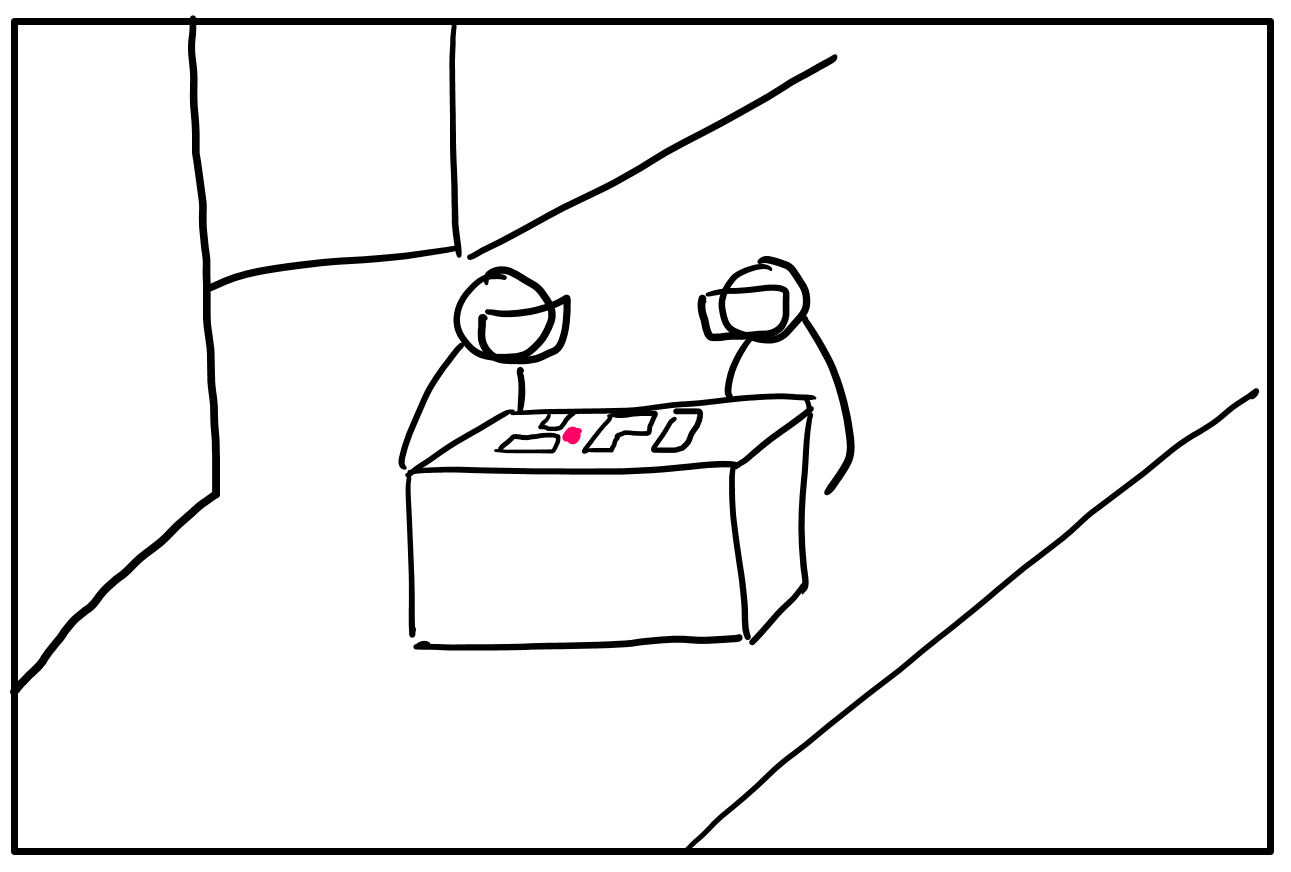
\includegraphics[scale=.2]{figures/comics/uncomfortable_collaboration.png}}
	\end{minipage}%
	\begin{minipage}{.25\linewidth}
		\centering
		\subfloat[]{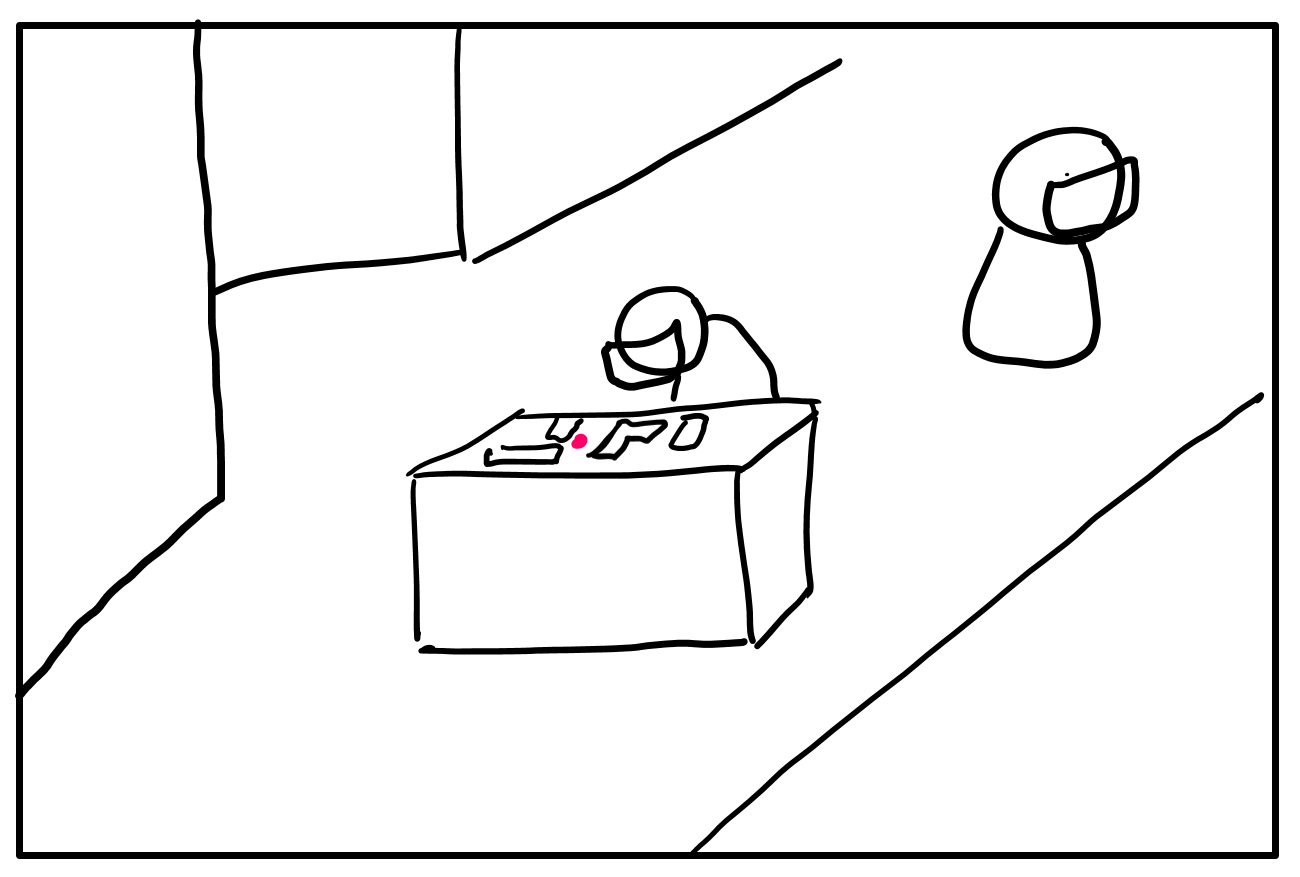
\includegraphics[scale=.2]{figures/comics/uncomfortable_collaboration2.png}}
	\end{minipage}%
	\begin{minipage}{.25\linewidth}
	\centering
	\subfloat[]{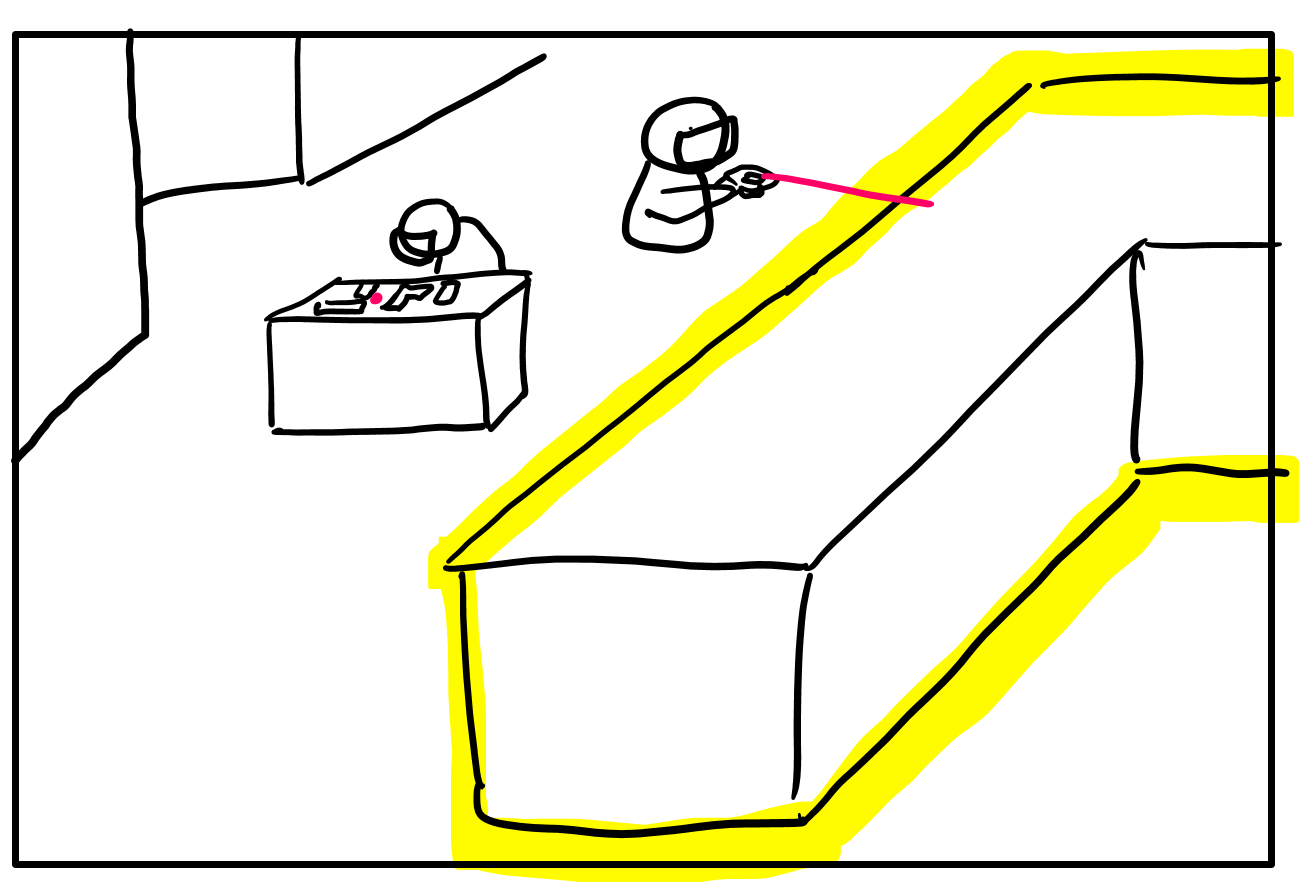
\includegraphics[scale=.2]{figures/comics/uncomfortable_collaboration3.png}}
	\end{minipage}
	
	\par\medskip
	\begin{minipage}{.25\linewidth}
		\centering
		\subfloat[]{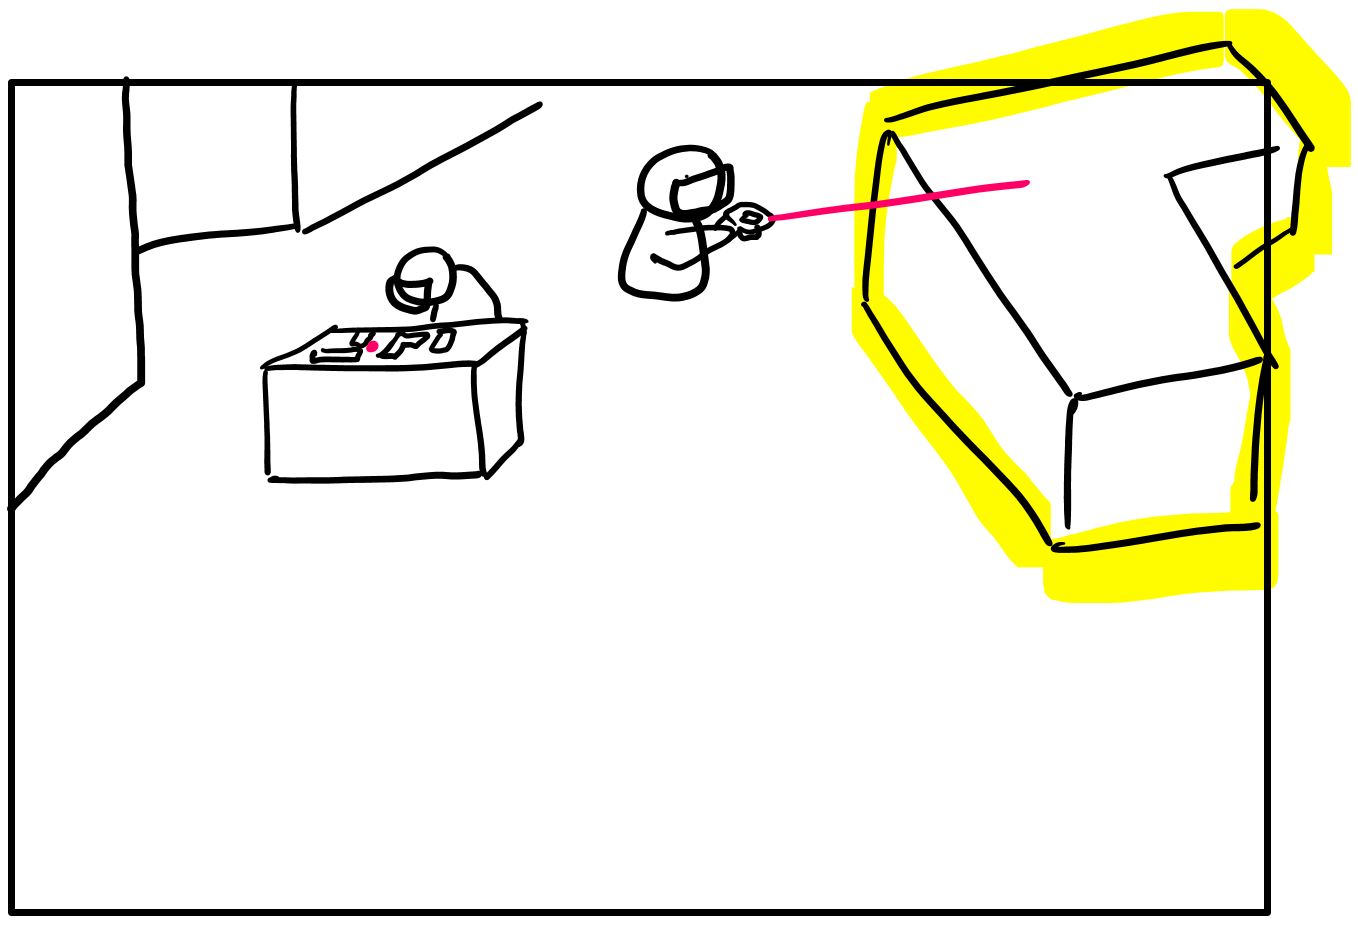
\includegraphics[scale=.2]{figures/comics/uncomfortable_collaboration4.png}}
	\end{minipage}%
	\begin{minipage}{.25\linewidth}
		\centering
		\subfloat[]{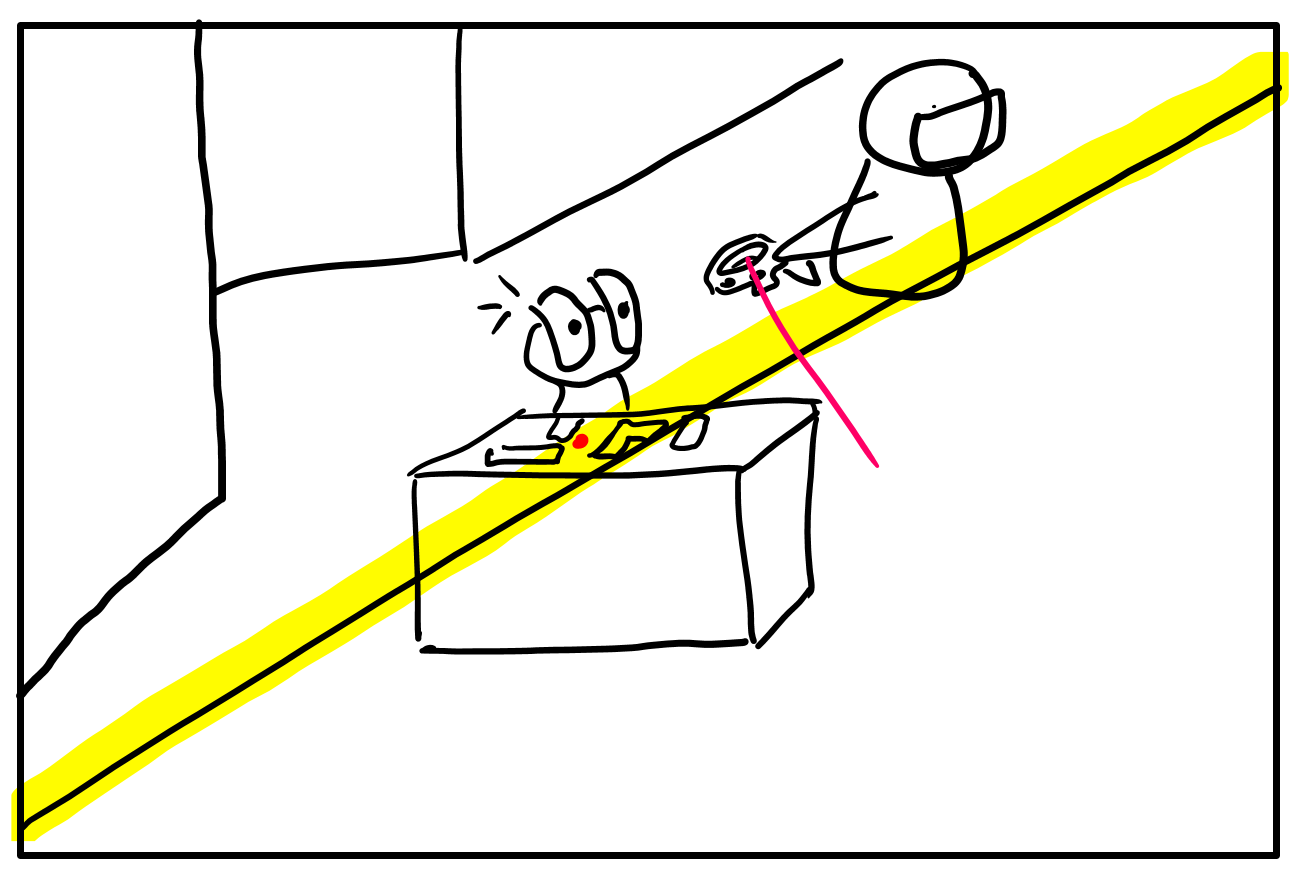
\includegraphics[scale=.2]{figures/comics/uncomfortable_collaboration5.png}}
	\end{minipage}%
	\begin{minipage}{.25\linewidth}
		\centering
		\subfloat[]{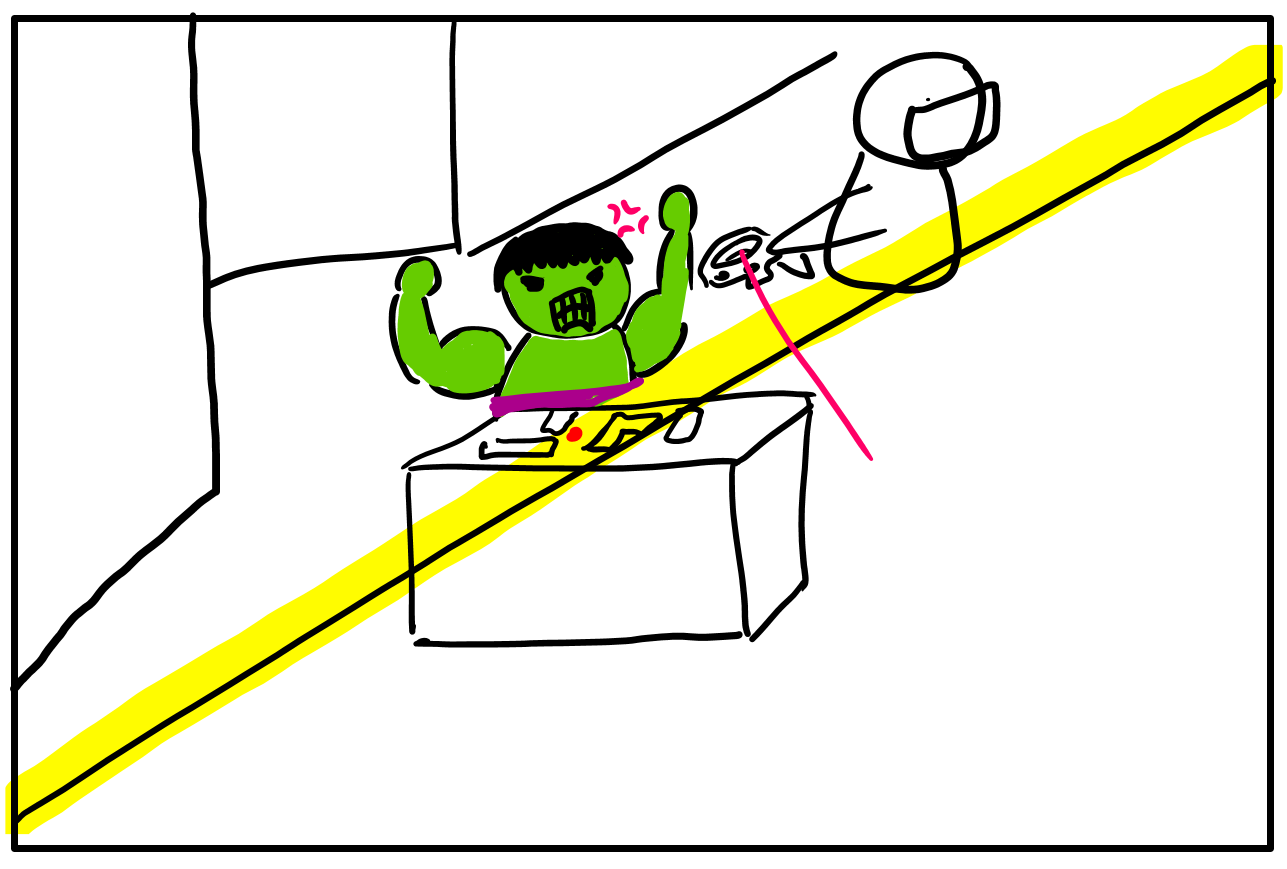
\includegraphics[scale=.2]{figures/comics/uncomfortable_collaboration6.png}}
	\end{minipage}
	
	\caption{Collaborators unaware of each other's actions}
	\label{fig:a1unawareofa2actions}
\end{figure}


%---------------Reference commands and structires

% \chapter{Introduction}\label{chapter:introduction}
% \section{Motivation: Teamwork is important. Creative thinking implies generation of ideas, collaboration, and communication. Virtual Reality (VR) is a great enhancement for creative thinking tool-set in architecture.}
%\subsection{Solution validation/evaluation in HCI: methods, and principles.}
\begin{comment}
Methodology: approach to solving the problem; chosen HCI methodology for the final evaluation - no idea
a. Chosen HCI evaluation methodology
\end{comment}


\begin{comment}
See~\autoref{tab:sample}, \autoref{fig:sample-drawing}, \autoref{fig:sample-plot}, \autoref{fig:sample-listing}.
\begin{table}[htpb]
  \caption[Example table]{An example for a simple table.}\label{tab:sample}
  \centering
  \begin{tabular}{l l l l}
    \toprule
      A & B & C & D \\
    \midrule
      1 & 2 & 1 & 2 \\
      2 & 3 & 2 & 3 \\
    \bottomrule
  \end{tabular}
\end{table}

\begin{figure}[htpb]
  \centering
  % This should probably go into a file in figures/
  \begin{tikzpicture}[node distance=3cm]
    \node (R0) {$R_1$};
    \node (R1) [right of=R0] {$R_2$};
    \node (R2) [below of=R1] {$R_4$};
    \node (R3) [below of=R0] {$R_3$};
    \node (R4) [right of=R1] {$R_5$};

    \path[every node]
      (R0) edge (R1)
      (R0) edge (R3)
      (R3) edge (R2)
      (R2) edge (R1)
      (R1) edge (R4);
  \end{tikzpicture}
  \caption[Example drawing]{An example for a simple drawing.}\label{fig:sample-drawing}
\end{figure}

\begin{figure}[htpb]
  \centering

  \pgfplotstableset{col sep=&, row sep=\\}
  % This should probably go into a file in data/
  \pgfplotstableread{
    a & b    \\
    1 & 1000 \\
    2 & 1500 \\
    3 & 1600 \\
  }\exampleA
  \pgfplotstableread{
    a & b    \\
    1 & 1200 \\
    2 & 800 \\
    3 & 1400 \\
  }\exampleB
  % This should probably go into a file in figures/
  \begin{tikzpicture}
    \begin{axis}[
        ymin=0,
        legend style={legend pos=south east},
        grid,
        thick,
        ylabel=Y,
        xlabel=X
      ]
      \addplot table[x=a, y=b]{\exampleA};
      \addlegendentry{Example A};
      \addplot table[x=a, y=b]{\exampleB};
      \addlegendentry{Example B};
    \end{axis}
  \end{tikzpicture}
  \caption[Example plot]{An example for a simple plot.}\label{fig:sample-plot}
\end{figure}

\begin{figure}[htpb]
  \centering
  \begin{tabular}{c}
  \begin{lstlisting}[language=SQL]
    SELECT * FROM tbl WHERE tbl.str = "str"
  \end{lstlisting}
  \end{tabular}
  \caption[Example listing]{An example for a source code listing.}\label{fig:sample-listing}
\end{figure}
\end{comment}